\section{Amélioration du prefetch de Blue Banana}
\subsection{Les changements introduits sur la version de Blue Banana}
\subsection{Les résultats et les observations sur le prefetch amélioré}
\subsection{Conclusion et perspectives}

Une des solutions est d'essayer de continuer le travail déjà réalisé dans Blue Banana~\cite{191}. L'objectif serait de rapatrier plus finement les données. Pour le moment, nous regardons juste les nœuds qui sont dans notre champs de vision (un cône) et qui ne sont ni trop loin, ni trop près. Mais il serait intéressant d'avoir plus d'informations sur les nœuds, comme leur direction ou leur vitesse par exemple. 
\par Actuellement un nœud, qui est dans l'état \textbf{T}(ravelling), va chercher des nœuds qui se trouvent sur la trajectoire probable de l'avatar, tant que son ensemble de voisins n'est pas plein. Ce mécanisme va donc rapatrier des données qui sont à bonne distance (pas trop près à cause des temps de communication). Un des risques est de rapatrier des nœuds qui sont inutiles si l'avatar, dont nous rapatrions les données, change de direction ou d'état. Le mécanisme existant ne va pas observer les différentes propriétés des nœuds (vitesse, direction, état, etc) et dans certains cas, il est possible qu'il rapatrie des nœuds qui viennent vers lui très rapidement et qui ne seront donc pas utiles.
\par L'idée est donc en plus de la distance avec le nœud de tester les différentes propriétés. Une solution serait peut être d'essayer de déterminer de façon simpliste les futures positions des nœuds et de tenir compte du couple vitesse/direction, pour mieux rapatrier les données. De plus, il faudrait chercher parmi des nœuds qui peuvent être hors du cône, mais sans trop chercher sinon trop de messages seraient émis.
\par  Nous pouvons voir un exemple de l'avantage de cet ajout (voir figure~\ref{prefetchav}), qui pourrait, par exemple, permettre l'ajout du nœud en rouge au lieu du vert.

	\begin{figure}[!h]
        \centering
        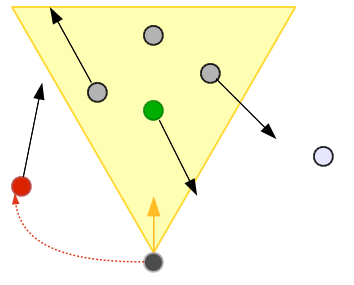
\includegraphics[scale=0.45]{./Ressources/Images/prefetchav.png}
        \caption{Exemple de gain possible pour le prefetching}
        \label{prefetchav}
        \end{figure}

\newpage
